\documentclass[11pt,fullpage]{article}
\newcommand{\mypara}[1]{\par \noindent {\bf #1}}
\newcommand{\beqa}{\begin{eqnarray}}
\newcommand{\eeqa}{\end{eqnarray}}
\newcommand{\beq}{\begin{equation}}
\newcommand{\eeq}{\end{equation}}
\newcommand{\ben}{\begin{enumerate}}
\newcommand{\een}{\end{enumerate}}
\newcommand{\bit}{\begin{itemize}}
\newcommand{\eit}{\end{itemize}}
\newcommand{\bi}{\begin{itemize} \item}
\newcommand{\ei}{\end{itemize}}
% \newcommand{\QED}{\hfill $\Box$}
% \newcommand{\QED}{\hfill {\bf QED}}
\newcommand{\tofix}[1]{ {\bf{[[$\Rightarrow$} #1]]} }
\newcommand{\ckm}{{$\surd$}}
\newcommand{\QED}{\hfill $\Box$ \hfill}
%\newtheorem{Definition}{Definition}[section]
%\newtheorem{defn}{Definition}[section]
%\newtheorem{Theorem}{Theorem}[section]
%\newtheorem{Proposition}[Theorem]{Proposition}
%\newtheorem{Corollary}[Theorem]{Corollary}
%\newtheorem{Example}{Example}[section]
%\newtheorem{Lemma}[Theorem]{Lemma}
%\newtheorem{Problem}{Problem}
%\newtheorem{problem}{Problem}
\newtheorem{Task}{Task}
\newtheorem{observation}{Observation}
%\newtheorem{Conjecture}{Conjecture}[section]
\newtheorem{Claim}{Claim}[section]
%\newenvironment{Proof}{\noindent{\bf Proof:}}{\QED}
\newenvironment{Note}{{\bf Note:}}{$\Box$\newline}

\newenvironment{Def} {\begin{Definition} \rm}{\end{Definition}}
\newenvironment{The} {\begin{Theorem} \rm} {\end{Theorem}}
\newenvironment{Exa} {\begin{Example} \rm} {$\Box$ \end{Example}}
\newenvironment{Pro} {\begin{Proposition} \rm} {\end{Proposition}}
\newenvironment{Cor} {\begin{Corollary} \rm} {\end{Corollary}}
% \newenvironment{Lem} {\begin{Lemma} \rm} {\end{Lemma}}
\newenvironment{Con} {\begin{Conjecture} \rm} {\end{Conjecture}}
% \newenvironment{Prob} {\begin{Problem} \rm} {\end{Problem}}
% \newenvironment{Prob} {\begin{Problem} } {\end{Problem}}

\newcommand{\begindef}{\begin{Definition} \rm}
\newcommand{\beginexa}{\begin{Example} \rm}
\newcommand{\beginthe}{\begin{Theorem} \rm}
\newcommand{\beginpro}{\begin{Proposition} \rm}
\newcommand{\beginlem}{\begin{Lemma} \rm}
\newcommand{\begincon}{\begin{Conjecture} \rm}
\newcommand{\begincor}{\begin{Corollary} \rm}
%\newcommand{\proof}{\noindent {\bf Proof}~:~}
\newcommand{\rem}{\noindent {\bf Remark}~:~}

\newcommand{\mat}[1]{{\bf #1}}   % matrix: bold

\newcommand{\vsp}{\vspace*{0.3cm}}
\newcommand{\vs}{\vspace*{1cm}}
\newcommand{\hs}{\hspace*{1cm}}
\newcommand{\pp}{\vspace{6 mm}}
\newcommand{\mywidth}{3in}


\def\br#1{\buildrel #1 \over \rightarrow}
\newcommand{\eat}[1]{}
\newcommand{\hide}[1]{\eat{#1}}
\newcommand{\keephide}[1]{\eat{#1}}
% \newcommand{\fighide}[1]{}
\newcommand{\fighide}[1]{#1}
% \newcommand{\old}[1]{{#1}}
% \newcommand{\new}[1]{{#1}}
% \newcommand{\defn}[1]{\underline{#1}}
% \newcommand{\defn}[1]{{\em #1}}
\newcommand{\manmonths}[1]{{\bf [#1 person-months]}}
\newcommand{\mm}{\manmonths}
% \newcommand{\reminder}[1]{ [[[ \marginpar{\mbox{$<==$}} #1 ]]] }
\newcommand{\remind}[1]{ {\bf *** #1 *** }}
%\newcommand{\comment}[1]{{\em\footnotesize #1}}
% \newcommand{\newcomment}[1]{{\em\footnotesize [** niko - drop? **] #1}}
% \newcommand{\comment}[1]{{\em\tiny #1}}
\newcommand{\attention}[1]{{\bf [** niko pls fix**] #1}}
% \newcommand{\comment}[1]{}

\newcommand{\question}[1]{{\em #1}}

% \newcommand{\patonly}[1]{{#1}}
% \newcommand{\paponly}[1]{{#1}}
% \newcommand{\tronly}[1]{{#1}}
% %%%%%%%%%%% set up for conditional text %%%%%%%%%%%%%%%
\newcommand{\eatreminders}{\renewcommand{\remind}[1]{}}
% \newcommand{\eatcomments}{\renewcommand{\comment}[1]{}}
% \newcommand{\eatpaper}{\renewcommand{\paponly}[1]{}}
% \newcommand{\eatpatent}{\renewcommand{\patonly}[1]{}}
% \newcommand{\eattr}{\renewcommand{\tronly}[1]{}}
%
% \newcommand{\finalpatent}{ \eatreminders \eatcomments \eatpaper }
% \newcommand{\draftpatent}{ \eatpaper }
%
% for ISR TR, with proofs etc
% \newcommand{\finaltr}{ \eatreminders \eatcomments \eatpaper }
% \newcommand{\drafttr}{ \eatpaper}
%
% for sigmod submission, with pointer to ISR TR
% \newcommand{\finalpaper}{ \eatreminders \eatcomments \eattr}
% \newcommand{\draftpaper}{ \eattr}
%%%%%%%%%%%%%%%%%%%%%%%%%%%%%%%%%%%%%%%%%%%%%%%%%%%%%%%%%%
% UNCOMMENT the appropriate next line, to prepare everything for the patent
% \draftpatent
% \finalpatent
%%%%%%%%%%%%%%%%%%%%%%%%%%%%%%%%%%%%%%%%%%%%%%%%%%%%%%%%%%
% UNCOMMENT the appropriate next line, to prepare everything for the ISR TR
% \drafttr
% \finaltr
%%%%%%%%%%%%%%%%%%%%%%%%%%%%%%%%%%%%%%%%%%%%%%%%%%%%%%%%%%
% UNCOMMENT the appropriate next line, to prepare everything for the paper
% \finalpaper
% \draftpaper
%%%%%%%%%%%%%end of setup for conditional text%%%%%%%%%%%%%%%
% \eatreminders

%%%%%%%%%%%%%%%%for VLDB/SIGMOD%%%%%%%%%%%%%%
\def\papernumber #1 raised #2 {
\vspace{-#2}
\vbox to 0pt{\hfill\framebox{\bf Paper Number #1}}
\vspace{#2}
}


\newcommand{\miobi}{\textsc{MIoBI}} % name of our method

\newcommand{\edgemake}{\textsc{MIoBI-MakeEdge}} % name of our method

\newcommand{\edgebreak}{\textsc{MIoBI-BreakEdge}} % name of our method
\newcommand{\nodebreak}{\textsc{MIoBI-BreakNode}} % name of our method
\newcommand{\myproof}{\textsc{Proof}}
\newcommand{\sproof}{\textsc{Proof Sketch}}
%\newcommand{\QED}{\hfill $\Box$ \hfill}
\newcommand{\A}{$\mathbf{A}$}
\newcommand{\uj}{$\mathbf{u}_j$}

\usepackage[letterpaper,margin=1.0in]{geometry}
\usepackage{afterpage}
\usepackage{subcaption}
\usepackage{subfig}
\usepackage{graphicx}
\usepackage{color}
\usepackage{appendix}
\usepackage{hyperref}
\usepackage{csvsimple}
\usepackage{lscape}

\begin{document}


\title{Towards a more transparent, complete and traceable data cleaning provenance model}
% \author{}
% \date{}
% \author{Lan Li}
% % \authornote{Authors are ordered by name.}
% %Both authors contributed equally to this research
% % \email{lanl2@illinois.edu}
% % \affiliation{
% %   \institution{University of Illinois, Urbana-Champaign}
% % }

\maketitle


\begin{abstract}
% provenance mining , without openrefine server running 
% reverse data cleaning 

OpenRefine is a powerful data cleaning toolkit, where it promises reproducibility by providing a reusable operation history, a JSON format recipe on GUI. This recipe's provenance information is not complete, transparent, and reusable enough, which brings up reproducibility issues. We finish three tasks in this paper:

1. Or2yw, a bridge between OpenRefine and YesWorkflow, is created by constructing the prospective provenance in OpenRefine recipe into the YesWorkflow diagram. This toolkit helps reveal the dependencies among operations in the recipe by scaling operations of OpenRefine into two types: inter-column and intra-column.

2. X-or2yw, a system that outputs a fine-grained and traceable hybrid provenance by combining the prospective provenance and retrospective provenance from OpenRefine workspace. This hybrid provenance records the computational processes and changes at the cell-level, improving the data cleaning provenance model's transparency and completeness. 

3. We also provide eight queries on hybrid provenance, including a quantitative review of the data cleaning task; output the complete provenance information at cell-level by revealing the dependency relationships; verify the traceability by
reversing the whole data cleaning task.

In this way, we could promise our data cleaning provenance model is more transparent, complete, and trustworthy. 



% through parsing project provenance archived from OpenRefine workspace, pairing merges the prospective provenance, from operation history, with retrospective provenance, by presenting actual changes of cells in the archive. 
% process level/ dependency --> cell 
% relate previous work --> now 
% DTA bridge 
% more high level : logic of or2yw ; throw away technical details

% 
% replay feature : x-or2yw
% given history of single cell --> process 
% 

 % later use DTA to verify/approve this 

% DTA: two kinds of transformation 

% We have constructed a user interface that transforms an OpenRefine recipe into a workflow diagram to make the protocol more transparent and understandable. OpenRefine recipes are ostensibly linear, but there are two levels of operations in OpenRefine, at 1) cell level and 2) schema level. It should be highlighted that when activities happened at the schema level, the structure of the whole workflow might change. In addition, it is hard to follow a lengthy and redundant recipe processes in the recipe. A high-level abstraction is needed to simplify those actions.

% The or2ywtool addresses these problems by automatically transform the original recipe in OpenRefine to a structuralized YesWorkflow model. YesWorkflow is a language-independent tool that can be used to visualize a workflow based on particular annotation and can be used to recover the information from the script. The the workflow model following transformation is more transparent than the JSON recipe. Also, it can provide implicit operation provenance information at both cell level and schema level in OpenRefine.




\end{abstract}

\section{Introduction}
OpenRefine is a popular data cleaning toolkit that allows users to do data transformations in a browser-based, spreadsheet-like GUI \cite{li2019towards}. Particularly, OpenRefine has a restricted interface to operate data cleaning workflow, combining the operations used in the transformation into a simple history list \cite{delpeuch2019complete}. This operation history provides both prospective and retrospective provenance. For prospective provenance, it collects the operations used in transformations and their arguments, i.e., prospective provenance needs to be captured before execution. Retrospective provenance is captured at runtime, such as the intermediate data produced \cite{murta2014noworkflow}.  

% the weakness of OpenRefine recipe
However, operation history in OpenRefine is of limited transparency. For operations in OpenRefine, some can change both the table's structure and value (e.g., the operation "Add column based on this column" will create a new column and new values based on the original schema ). The other type of operations will only affect the cell values (e.g., operation "To lowercase" will change cells' values in this column to fit for the pattern). Or2yw toolkit scales dependency on column level, where the former inter-column transformations as rigid transformations, the latter intra-column ones as geometry transformations \cite{nunez2020first}.
Geometry transformation will "break" the data lineage of the original table. Therefore, it is not easy to trace the lineage from a provenance perspective if there are breakpoints in the processes. Or2yw toolkit could help transpose operation history into the Yesworkflow diagram, helping return each operation's dependency \cite{mcphillips2015yesworkflow}.

Based on previous work, we find the operation history in OpenRefine is not complete at least in two ways: functions missing in operation \textit{Cluster and Edit}; mass cell changes, e.g., uppercase the values in a column, and \textit{Single Cell Edit} are not captured. Regarding the retrospective provenance, reversible functions cover complete information to promise backward compatibility, which irreversible ones need additional provenance information of past values \cite{nunez2020first}.

We observe the workspace in OpenRefine, within which it manages all of the projects \cite{OpenRefine}. All changes to the project's data are supposed to be tracked, where the sub-directory \textit{history} store diffs, actual changes after applying the operation, the sub-directory \textit{data} store column model, processes (i.e., operations and history pairs), and current status of the dataset. The provenance stored in \textit{history} and \textit{data} are neither complete to some extent. For \textit{history}, there is no computational method recorded. For instance, the changes caused by intra-column transformation would be saved as "MassCellChange" in \textit{history}. We do not know what this applied operation is. In \textit{data}, the operation applied would be recorded, while changes at cell level are not recorded. 

As a result, we combine the provenance from change objects and processes by pairing the history entries, where the history entry is the id of every transformation, which is unique. The provenance at \textit{history} is in the text file, hard to trace. To make the hybrid provenance human-readable and easy to query, we transpose the text file into JSON format and concatenate JSON type provenance in \textit{data}. 

We provide eight queries on hybrid provenance, given a cell with a row index and column index, including:
1. List all of the changes on this cell
2. List all of the operations applied to this cell
3. Count how many changes on this cell
4. Count how many operations applied on this cell
5. Count how many cells have been changed
6. List all of the cells which get changed
7. Reverse the data cleaning task and return the original cell value
8. List the provenance of this single cell

The first four queries are for distinguishing the "change" and "operation," where operation applies on the whole column, but not all are affected. In this situation, there is no change caused by this cell. 

Query 5 and 6 are to summarize how many efforts are put into this data cleaning task. 

Query 7 is to reverse the whole data cleaning task by this hybrid provenance. By comparing the input original cell value with the result, we could promise this data cleaning task is compatible and trustworthy. 

The last query is to discriminate "provenance" and "changes," where the full provenance of a cell should be the history of the cell changes composed with a history of depending multiple other cells\cite{nunez2020first}. With the help of dependency information by or2yw toolkit, we could return the cell's complete provenance. 


\section{Background}
% reproducibility issue
There are over than 70 percent of scientists failed to reproduce other people's work, and more than half of scientists cannot reproduce their own work \cite{baker2016reproducibility}. "Reproducibility crisis" often refers to the inconsistency in results across studies \cite{samsa2019guide}. Discussion about reproducibility should consider repeatability of data management and analysis with an identical answer, where data management is to reconstruct the original data and prepare it for further analysis. Data cleaning is one essential part of the data management, through which data errors would be addressed and fixed. An adopted taxonomy that covers all the error types is proposed; four types of data errors are categorized, one of which is named outliers classified as quantitative, the other includes duplicates, rule violations, and pattern violations are classified as qualitative ones \cite{abedjan2016detecting}. Different data cleaning tools will focus on different data errors, trying multiple approaches to decide on the estimated values that best support the hypothesis with rationale.

For preclinical research, an auditable record of original data is required for reproducible, including the rationale for data cleaning and retaining the analysis programs. As the dataset size is increasing, a formal software-based system for data cleaning and management is needed to create an analysis file, which is reproducible documentation of the data analysis \cite{samsa2019guide}. 
% Hybrid provenance is significant and necessary 
There are two forms of provenance, prospective and retrospective. \textit{prospective provenance} captures the procedure of computational processes, working as a recipe that must be followed to reproduce the data product or class of data products. \textit{retrospective provenance} captures the executed products during the computation, i.e., it's a detailed log of the computational task \cite{freire2008provenance}. Combining retrospective and prospective provenance can produce scientifically significant hybrid provenance representations of the computational histories of data produced during a script run \cite{zhang2017revealing}. This integration of provenance can both reveal the overall history of a script run and also the fine-grained history of particular script products. 

% hybrid provenance - cell level could fix reproducibility issue
Data cleaning is noteworthy in data science. Scientific reproducibility highly depends on a well-curated dataset, where it means specific data storage format specification, no lexico-graphic errors, or miscategorized entities, adequate representation of missing data inferred by the valid existing data \cite{nunez2020first}.  Data cleaning tools such as OpenRefine provides a recipe recording the \textit{operation history} in JSON format. This recipe is supposed to be reused and reproduces the data cleaning workflow, where it captures the incomplete computational steps as well as partial execution products, i.e., we named it incomplete hybrid provenance. The paper uncovers the history of individual cell contents, i.e., it provides a model that promotes cells as first-class citizens in the data cleaning workflow \cite{nunez2020first}. This cell-level retrospective provenance could answer questions about how a given value in a cell came to be, and what its individual operation history was. 






\section{Prototype}
\label{prototype}
\subsection{Or2yw Tool}
The or2yw toolkit could generate three modes; Yesworkflow is used to construct the JSON-format OpenRefine recipe into the data cleaning diagram. OpenRefine transformations will be extracted as a process. The corresponding values of parameters in transformations are as input parameters in the Yesworkflow system. We provide three modes, including sequential mode, parallel mode, and merge mode. The sequential mode is by following the OpenRefine recipe, step by step. Compared with Sequential mode, the parallel mode would be closer to the dependency relationship among transformations in OpenRefine. Taken the differences of dependencies between columns and inter the same column into consideration, we introduce this "parallel" conception into the data cleaning workflow. In other words, Given a transformation T{$_1$} on column C{$_1$}, if the afterward transformation T{$_x$} also works on column C{$_1$}, then this following transformation is supposed to be dependent on the effect of T{$_1$}. In this situation, the structure of T{$_x$} and T{$_1$} would be sequential. On the other side, if the transformation  T{$_x$} applies to a different column, named column C{$_2$}. As the column C{$_2$} is independent of column C{$_1$}, the  T{$_x$} should be independent with the effect of T{$_1$}, and the structure of T{$_x$} and T{$_1$} would be parallel. With this dependency recovery, the data cleaning workflow in OpenRefine would be much more transparent. As defined in Data Transformation Algebra, Geometry transformation in openRefine would "break" the existing dependency relationships by creating new columns or deleting old columns \cite{nunez2020first}. To get the full provenance information on some column, especially the single cell's provenance, we need to make the dependency information in the data cleaning workflow explicit. 


\subsection{Hybrid Provenance}
We propose a hybrid provenance to fix the transparency and dependency issues with OpenRefine recipe \cite{li2019towards}. There is a $workspace$ in OpenRefine architecture, which has metadata file, and complete provenance files, including $data.txt$ and $history$ folder. 

Provenance information in OpenRefine recipe is the subset of provenance in $data.txt$, for the missing provenance information is recorded in $data.txt$, e.g., the single edit transformation is not recorded in OpenRefine recipe; the other significant extra provenance information provided by $data.txt$ is the history ID, created when data transformation is applied, and the time stamp when processes this transformation.  Thus, we could infer from provenance in $data.txt$ as $P_\mathcal{D}$ to provenance in OpenRefine Recipe $P_\mathcal{OR}$.

\begin{equation}
    P_\mathcal{D} \mapsto P_\mathcal{OR}
\end{equation}

The granularity of provenance information in $data.txt$ and $history$ folder is different; the preceding is of schema level, the succeeding is of cell level. For the missing provenance on the cell level, such as \textit{Single-Edit} transformation, $history$ records the row index, column index, old value, and new value.
For transformations which might bring up dependency broken issues, e.g. \textit{Split-Column} transformation, $history$ records the new generated columns,both values and fields names. Generally speaking, $history$ could fix the partial transparency issues as well as dependency issues. The partial here is because $data.txt$ will record the prospective provenance of transformations, namely transformation function types, function methods, function parameters, while $history$ does not log provenance information that is mandatory for achieving reproducibility and transparency. 

The sharing information between $data.txt$ and $history$ folder is the history ID. We choose to amalgamate the provenance both at $data.txt$ and $history$ through pairing provenance from two ends by history ID, where we named it hybrid provenance. Here provenance in $history$ is rewritten in JSON format following the data types in $data.txt$. JSON is easily readable both for human and machine, uncomplicated for tracing. Then we did several queries on this hybrid provenance to promise its extended transparency, reputability, and completeness \ref{fig:hp_archi}. 

\begin{figure}
\centering
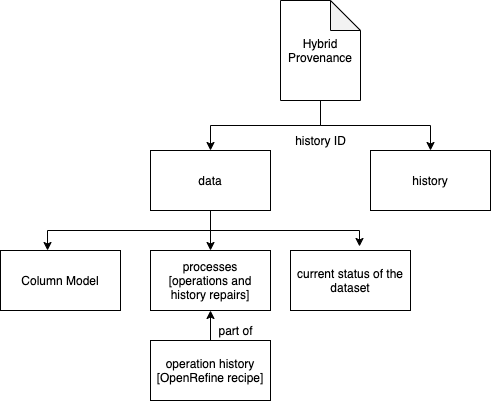
\includegraphics[width=8cm]{Figure/hybrid_provenance_archi.png}
\caption{Architecture of hybrid provenance}
\label{fig:hp_archi}
\end{figure}


\section{Use Case}
\label{usecase}
\subsection{Or2yw Toolkit}
We use dataset $menu.csv$ from The New York Public Library, where it is a mix of simple bibliographic description of the menus (created by The New York Public Library) and the culinary and economic content of the menus themselves (transcribed by users)\cite{whatsonmenu}. We could expect how low the dataset's data quality could be that integrates manual and systematic input.

There are three modes in or2yw toolkit, including sequential, parallel and merge. Sequential mode is by directly translate the data cleaning workflow from the original JSON file (see Figure \ref{fig:recipe}), step by step without considering the dependency relationships among operations. 

Compared with Sequential mode, the parallel mode aims to recover the dependencies in the recipe on column level. Here are certain conditions that define parallel operations. 

\textbf{Parallel Node}: Operations in OpenRefine are applied row-wise and are stateless: no state is maintained among the processing of rows \cite{delpeuch2019complete}. It is thus easy to parallelize the operations if the operations are executed under different columns, as they amount to a pure map on the list of rows. Operations on different columns are expected to be mutually exclusive and not affect each other, while any actions on the same column following those parallel operations will be executed sequentially. 

\textbf{Join Node}: Two or more parallel operations will be joined together if there is one operation that combines two or more columns as input parameter in the recipe. The joined operation will be executed respectively to the latest transaction on each column preceding this operation. E.g. operation $Add column based on this column...$ allows users to concatenate multiple columns and create a new column. 

\textbf{Split Node}: One or more new nodes will be generated if an operation produces multiple columns. The new generated columns are mutually exclusive, therefore, they could be seen as parallel node.  


\begin{figure}
\centering
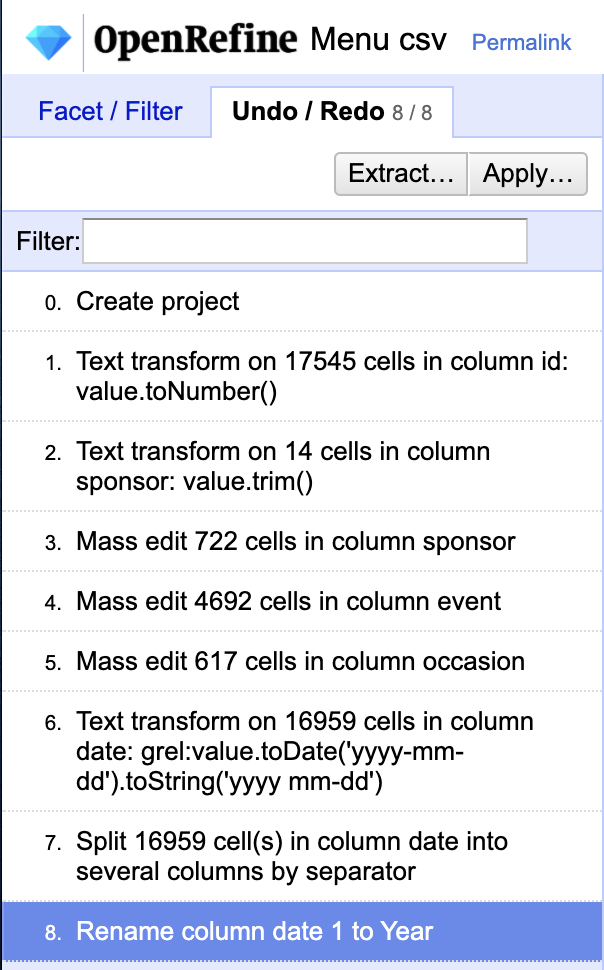
\includegraphics[width=5cm]{Figure/OR_recipe.png}
\caption{Operation History in OpenRefine}
\label{fig:recipe}
\end{figure}

\afterpage{%
\begin{figure}
  \centering
  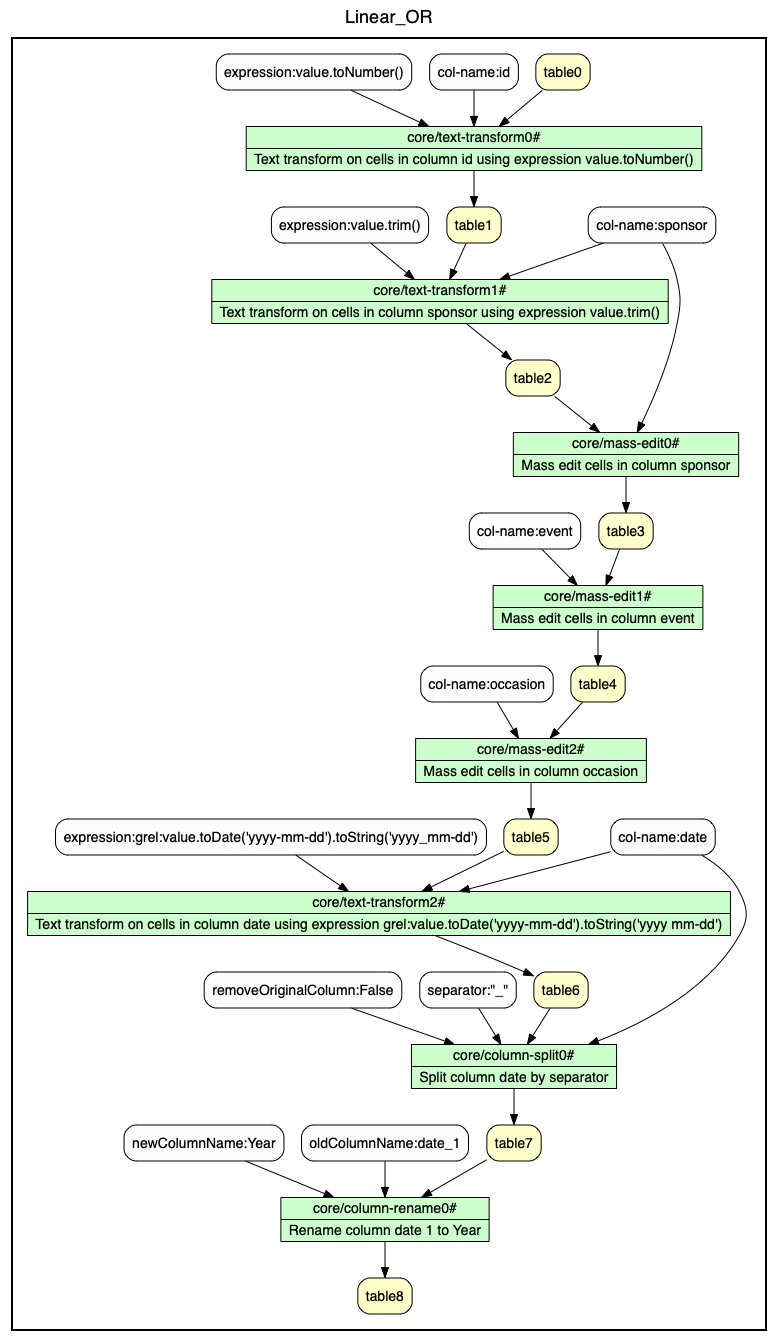
\includegraphics[width=0.7\linewidth]{Figure/dc_linear.png}
  \caption{Sequential: There are eight steps in the recipe, green box stands for the transformations, white box stands for input parameters, and yellow box represents the data stream.}
  \label{fig:sub1}
\end{figure}
\clearpage
}


\begin{landscape}

\afterpage{%
\begin{figure}
  \centering
  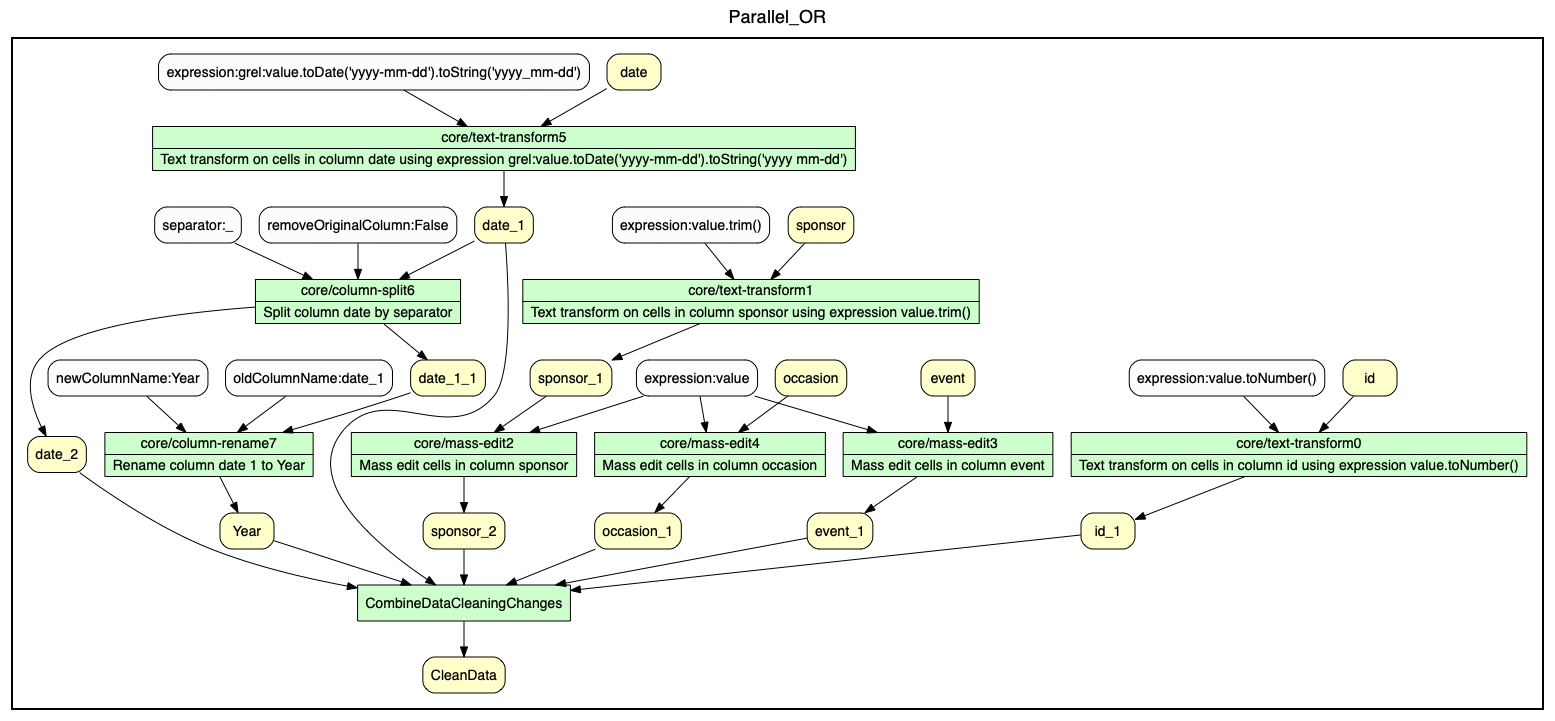
\includegraphics[width=1\linewidth, scale =1]{Figure/dc_parallel.png}
  \caption{Parallel: Transformations on column $date$, $sponsor$, $occasion$, $event$ and $id$ are parallel nodes; Split node generates by applying column-split on $date\_1$, where there are two new nodes generated, $date\_1\_1$ and $date\_2$; In the final status, $CombineDataCleaningChanges$ will merge all of the changed columns, where we could see this as Join node. }
  \label{fig:sub2}
\end{figure}
\clearpage
}
\end{landscape}


%\caption{Sequential VS Parallel: From syntactic perspective, Sequential mode is like depth-first Tree, while Parallel tends to be breadth-first tree. Parallel mode could illustrates concurrency better.}
%\label{fig:test}
%\end{figure}

%\begin{figure}

%\begin{subfigure}{.5\textwidth}
%  \centering
%  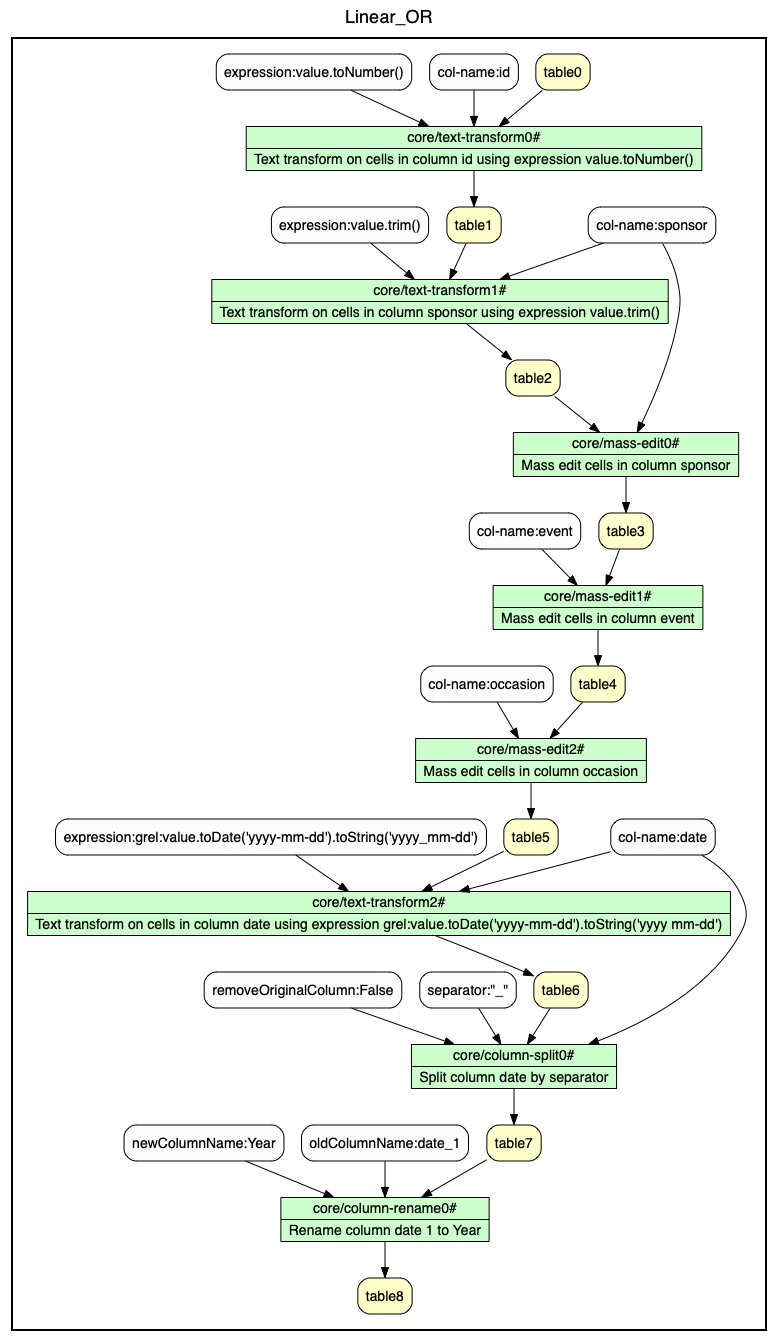
\includegraphics[width=0.6\linewidth]{Figure/dc_linear.png}
%  \caption{Sequential: There are eight steps in the recipe, green box stands for the transformations, white box %stands for input parameters, and yellow box represents the data stream.}
 % \label{fig:sub1}
%\end{subfigure}%
%\begin{subfigure}{.4\textwidth}
%  \centering
%  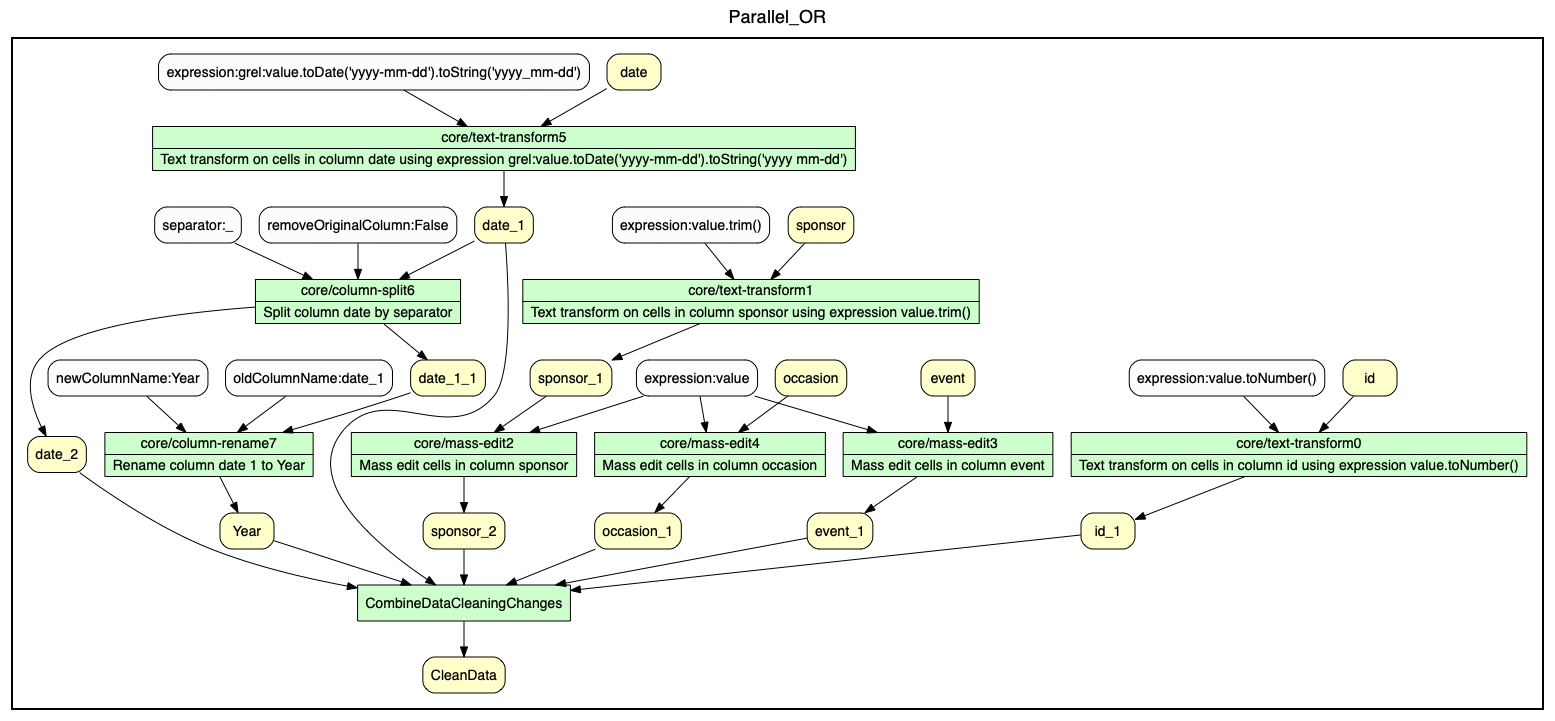
\includegraphics[width=1.6\linewidth, scale =1]{Figure/dc_parallel.png}
%  \caption{Parallel: Transformations on column $date$, $sponsor$, $occasion$, $event$ and $id$ are parallel nodes; Split node generates by applying column-split on $date\_1$, where there are two new nodes generated, $date\_1\_1$ and $date\_2$; In the final status, $CombineDataCleaningChanges$ will merge all of the changed columns, where we could see this as Join node. }
%  \label{fig:sub2}
%\end{subfigure}
%\caption{Sequential VS Parallel: From syntactic perspective, Sequential mode is like depth-first Tree, while Parallel tends to be breadth-first tree. Parallel mode could illustrates concurrency better.}
%\label{fig:test}
%\end{figure}


The merge mode is mainly dealing with recipe which is of high volume or has many "redundant" operations. Although the or2yw toolkit can produce the workflow, the output has so many nodes that it is too messy and complicated to trace. For this reason, we propose a method to merge those redundancies, where redundancy means same operations with different parameters applying on the same column. By examining the column name, or2yw toolkit will find the same operations that are executed sequentially and join them together to produce only one operation node. A separated text file is provided representing a sub-workflow that contains detailed operations and stores the parameter information as a node description. With this approach, we can produce a typical workflow for a large process with redundant operations without losing the provenance. 



\subsection{Queries with Hybrid Provenance}

Through pairing the history ID between $data.txt$ and $hisotry$ folders, we could get hybrid provenance (See Figure \ref{fig:hp process}).



\begin{figure}

\begin{subfigure}{.5\textwidth}
  \centering
  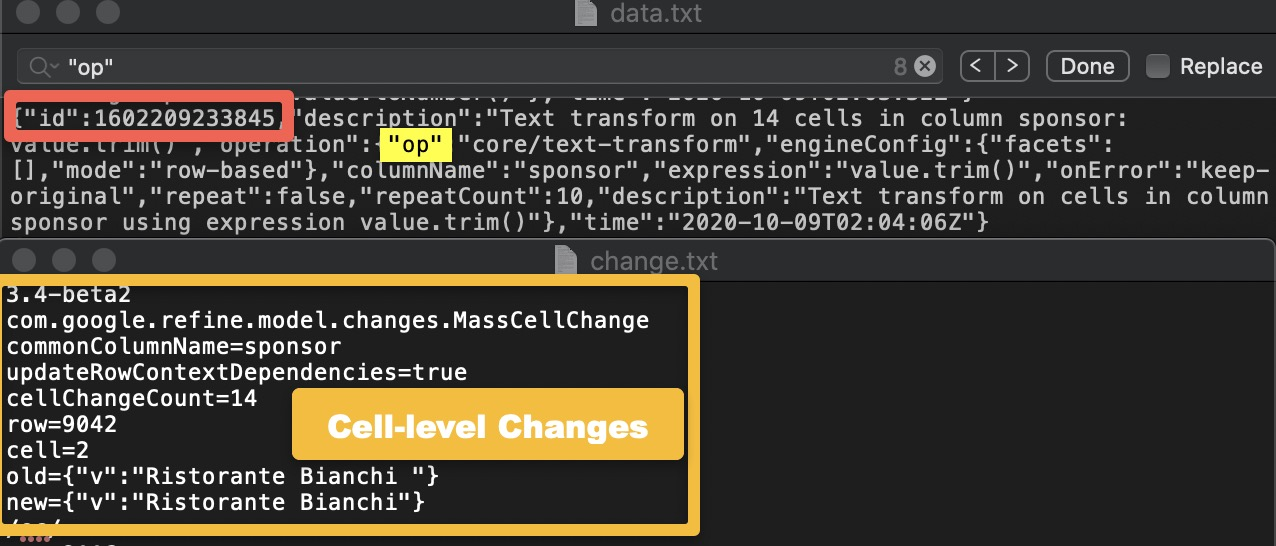
\includegraphics[width=1\linewidth, scale=1]{Figure/data-his-pair.jpeg}
  \caption{Red box is the history ID in $data.txt$, yellow box includes the cell-level changes from $history$. Provenance at cell-level would be rewritten into JSON file, and combined with changes in $data.txt$. In this way, we could get hybrid provenance (see Figure \ref{fig:hp})}
  \label{fig:pair}
\end{subfigure}%
\hspace{1em}
\begin{subfigure}{.4\textwidth}
  \centering
  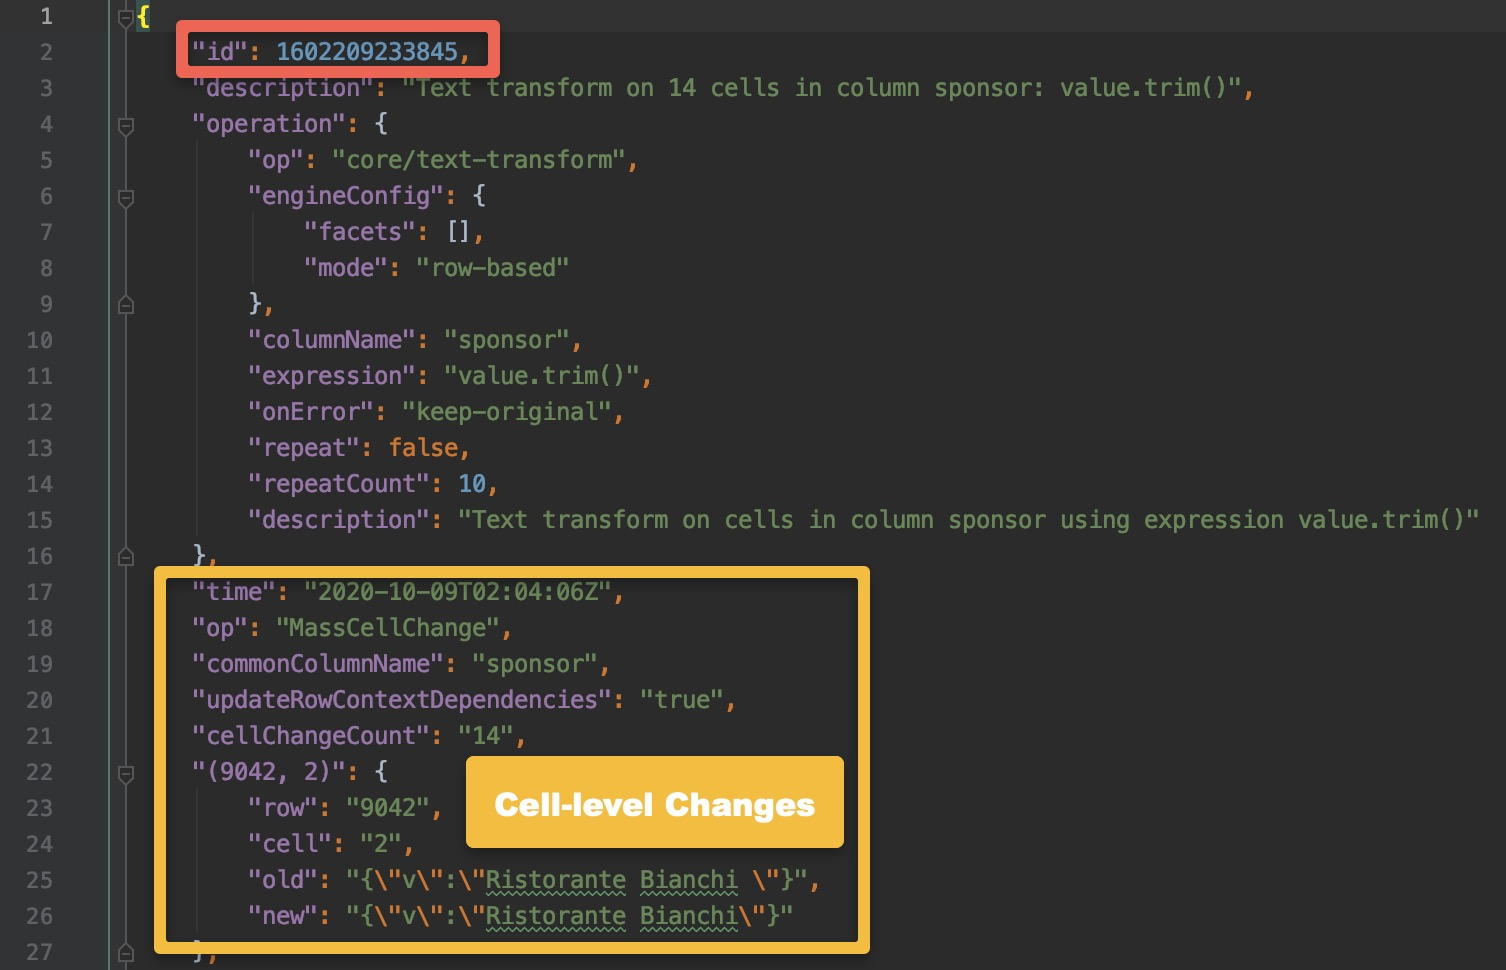
\includegraphics[width=1\linewidth, scale =0.8]{Figure/Hybrid.jpeg}
  \caption{Hybrid provenance is in JSON format, composed of provenance information in operation-level from $data.txt$ and in cell-level from $history$. }
  \label{fig:hp}
\end{subfigure}
\caption{}
\label{fig:hp process}
\end{figure}


Given the provided hybrid provenance, we would like to ask specific
questions about what its individual operation history was, how a given value in a cell came to be, reverse the data cleaning if we could get the original value. Metaphorically, we illustrate the data cleaning workflow as a collection of leaves along a flowing river: leaves are the cells in the dataset as the first-class citizens with an interesting life of their own. Many of the leaves will be lost, but for the surviving ones we are supposed to be able to tell their history as long as we know their traces in the river \cite{nunez2020first}.

In the query table (See Table \ref{tab:hybrid_prov}), there are eight queries in total. Consider given a "weird" cell value after a chain of data cleaning steps, there are some possible situations. Case one, there is no operation applied on this single cell, data quality is upstream and data is not cleaned thoroughly. Case two, an inappropriate cluster function is applied and errors are introduced. Case three, even if the value appears to be unchanged from the input, while multiple operations have been applied and the effects can be offset each other. For the previous two cases, it would be easy to trace the provenance with the help of OpenRefine recipe. Nevertheless, for the last case, the data was in fact changed during the data cleaning workflow multiple times and ended up having the same value. Fine-grained cell-level provenance information is required to inspect what really happened. Query 1,2 and 8 will return the story of a single cell. Query 3,4,6 and 7 are the quantitative analysis. Query 5 reverse the data cleaning task and return the derivation of cell value. 



\begin{table}
    \centering
    \begin{tabular}{c|c}
    \hline
    \textbf{Query Description} & \textbf{Query Command} \\
    \hline
    List all of changes applied on the given cell & changes-single-cell \\
    \hline
    List all of operations applied on the given cell & operations-single-cell \\
    \hline
    Count how many changes applied on the given cell & count-changes-single-cell \\
    \hline
    Count how many operations applied on the given cell & count-operation-single-cell \\
    \hline
    Reverse the data cleaning task and return the original cell value & reverse-data \\
    \hline
    List all of the cells indexes which get changed & list-changed-cells \\
    \hline
    Count how many cells have been changed & count-changed-cells \\
    \hline
    Provenance of the given cell & prov-single-cell \\
    \hline
    Return the answer of the whole query table & merge \\
    \hline
    \end{tabular}
    \caption{Hybrid Provenance Query table}
    \label{tab:hybrid_prov}
\end{table}





\section{Discussion and Conclusion}
A scientific workflow system is supposed to capture metadata indicating which specific data products and tools are used to create a derived data products, and automatically record the sequence of applied processes, parameter settings, and intermediate data products \cite{ludascher2006scientific}. Hybrid provenance proposed by this paper is composed of computational steps, metadata including transformation functions and parameter settings, and log of intermediate cell values. By querying the hybrid provenance at the cell level, we promise its completeness, transparency. Reversibility of the whole data cleaning task promises the reproducibility and trustworthiness of this hybrid provenance. From dataset history to cell provenance, the hybrid provenance repairs the broken dependency issue. Or2yw toolkit, a bridge between the data cleaning recipe in OpenRefine and Yesworkflow system, helps reveal the recipe's dependency relationships. 

%%
%% The next two lines define the bibliography style to be used, and
%% the bibliography file.
\bibliographystyle{plain}
\bibliography{ref}

\section{Appendix}

\begin{table}[h]
    \centering
    \small
    \csvautotabular{email.csv}
    \caption{Minimum Dataset for Email Onboarding from Staffbase}
    \label{tab:example_dataset}
\end{table}



In the appendix, we use the example from \cite{nunez2020first} as a demo of querying hybrid provenance.  The dataset is the Minimum Dataset for Email Onboarding(Table \ref{tab:example_dataset}).

We reproduce the data cleaning task with OpenRefine, see Figure \ref{fig:reproduce}. There are five steps in total:

1. We need to extract users' names from 'Login email' without '@' and domain part.

2. We transform data types to numeric in the column Identifier, and as the identifier starts from 0 instead of 1, we delete one each.

3. We add one more column named 'group' based on the value in 'Identifier.' The fourth and fifth is to uppercase the strings in column 'First name' and 'Last name.' 

\begin{figure}
\centering
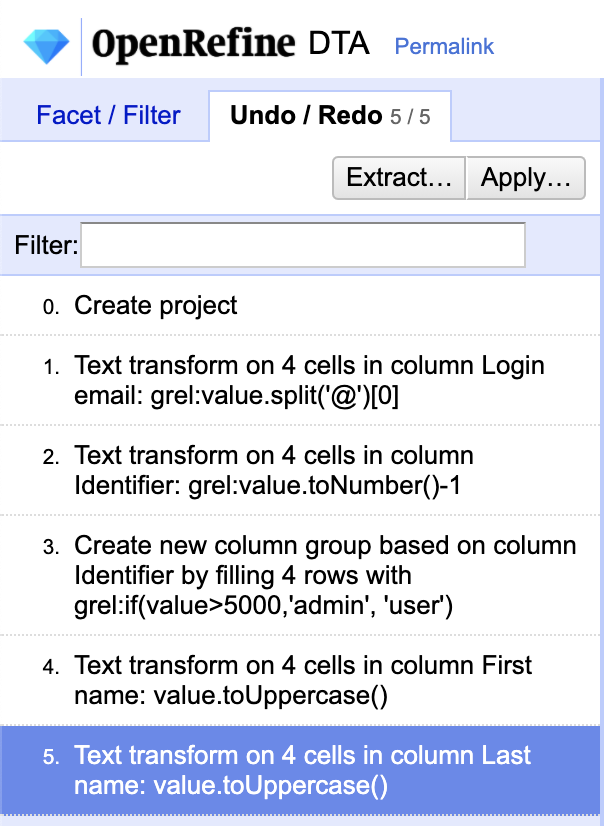
\includegraphics[width=5cm]{Figure/DTA_demo.png}
\caption{Reproduce data cleaning task}
\label{fig:reproduce}
\end{figure}


\subsection{\textbf{The history of three cells}}

We use the query table to reconstruct the operation history of three cells: (1,1), (2,2), and (3,5). According to Table \ref{tab:hybrid_prov}, input the arguments including, hybrid provenance, row index, column index and command $prov-single-cell$, then output the results saving in the result folder, see the Table \ref{tab:DTA_usecase}. (NB: the index starts from 0 in the python program, while for the table, it starts from 1. Therefore, the corresponding provenance is cell at (0,0), (1,1) and (2,4)). 

In the result table \ref{tab:DTA_usecase}, the first column is the cell index, which we want to ask for the provenance. The second column displays the provenance file; the third and fourth columns show the changes of each step. The last column represents the provenance index, which stands for dependency. As we could find, cell at (0,0) and (1,1) are dependent on themselves, while for the cell at (2,4), it has another dependent column. That is because in the data cleaning step 3, this new column 'group,' located in column index 4, is created based on the column $Identifier$, which is located in column index 1.  

In this way, we have verified that hybrid provenance is complete and transparent, providing us with the cell-level changes. On the other side, this query-based provenance helps reveal the dependency information. 

\begin{table}
    \centering
    \begin{tabular}{c|c|c|c|c}
    \hline
    \textbf{Index} & Provenance File & Old Value & New Value & Provenance Index \\
    \hline
    (0,0) & 'hybrid1' & 'laura@example.com' & 'laura' & (0,0) \\
    \hline
    (1,1) & 'hybrid2' & ' 4081'& 4080 & (1,1) \\
    \hline
    (2,4) & 'hybrid2' & ' 9346' & 9345 & (2,1) \\
     & 'hybrid3' & None & 'admin' & (2,4) \\
    \hline
    \end{tabular}
    \caption{Result of Provenance for three cells}
    \label{tab:DTA_usecase}
\end{table}





\footnote{See: \url{https://github.com/LanLi2017/X_or2yw}}

\end{document}

%%
%% End of file `sample-authordraft.tex'.
